% =========================================================
% TITLE PAGE
% =========================================================

\begin{frame}[plain]

    \networkbackground

    \vspace{1cm}

    {\small
    \textcolor{blueColor}{
        DOKTORSKA DISERTACIJA
    }}

    \vspace{0.5cm}

    {\huge
    \textcolor{blueColor}{
    Unapređenje distribuirane platforme za e-trgovinu na javnoj blockchain mreži u cilju minimizacije računarskog napora prilikom izvršavanja transakcija
    }}

    \vspace{0.35cm}

    \textcolor{blueColor}{\rule{2.0cm}{1pt}}

    \begin{columns}[t]

        \begin{column}{0.48\textwidth}

            \textcolor{whiteColor}{\textbf{Mentor:}\\
            prof. dr Mladen Veinović}

        \end{column}

        \begin{column}{0.48\textwidth}

            \raggedleft

            \textcolor{whiteColor}{\textbf{Student:}\\
            Vukašin S. Tasić 2020/460030}

        \end{column}

    \end{columns}

    \begin{center}
        {\Large
        \textcolor{whiteColor}{
            Univerzitet Singidunum
        }}
    \end{center}

\end{frame}

% =========================================================
% SLIDE 2
% =========================================================

\begin{frame}{Savremeni informacioni sistemi}

Elektronska trgovina predstavlja prodaju ili kupovinu robe i usluga realizovanu putem računarskih mreža korišćenjem metoda posebno projektovanih za prijem ili izdavanje porudžbina.

\metodologijaCilj{Formalizacija referentog modela elektronske trgovine kroz identifikaciju ključnih elemenata sistema, radi omogućavanja analize dizajna sistema elektronske trgovine.}


\begin{figure}[ht]
    \centering
    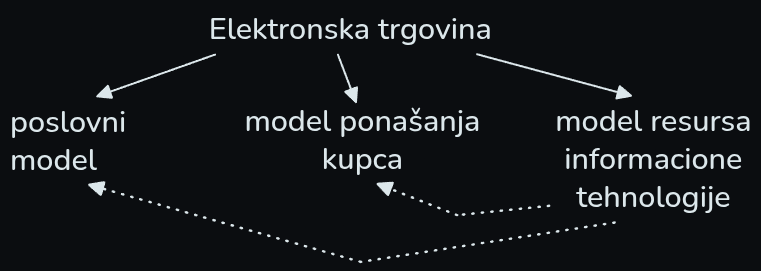
\includegraphics[width=0.6\textwidth]{slide2.png}
\end{figure}

\end{frame}

% =========================================================
% SLIDE 3
% =========================================================

\begin{frame}{Savremeni informacioni sistemi}

\metodologijaProblem{} Savremeni informacioni sistemi, uključujući sisteme elektronske trgovine, dominantno se zasnivaju na centralizovanom modelu u kojem se poverenje delegira trećim stranama sa kontrolom nad podacima i pravilima sistema.

To smanjuje autonomiju korisnika i stvara asimetriju moći, koja se ogleda u: \redColor{algoritamskoj kontroli}, \redColor{cenzuri i kontroli pristupa}, \redColor{koncentraciji moći}, \redColor{nadzornom kapitalizmu} i \redColor{zloupotrebi ličnih podataka}.

\metodologijaCilj{Analiza savremenih informacionih sistema elektronske trgovine, sa ciljem identifikacije njihovih ograničenja i implicitnih pretpostavki u pogledu poverenja i upravljanja podacima korisnika.}

\end{frame}

% =========================================================
% SLIDE 4
% =========================================================

\begin{frame}{Savremeni informacioni sistemi}

\vspace{-0.35cm}

\metodologijaProblem{} Uklanjanje centralizovanog autoriteta uvodi mogućnost neispravnog ili malicioznog ponašanja pojedinih učesnika, pri čemu sistem mora očuvati konzistentnost.

Decentralizacija zahteva \blueColor{otvoren sistem} bez \redColor{centralne kontrole} ili jedne tačke otkaza.

\metodologijaCilj{Uvođenje i formalizacija pojma decentralizacije kao proširenja klasične sociotehničke paradigme informacionih sistema.}

\vspace{-0.7cm}

\begin{figure}[ht]
\centering

\subfloat[Centralizovan]{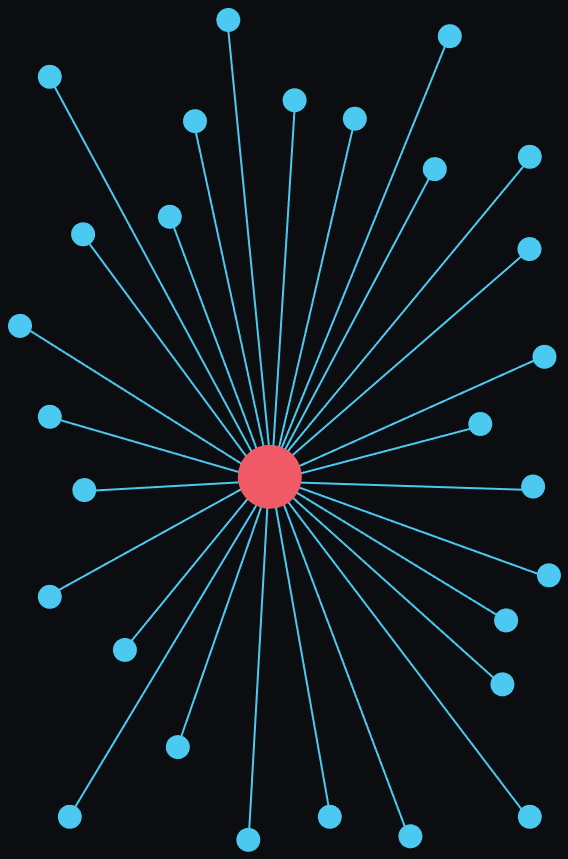
\includegraphics[width=0.19\textwidth]{slide4a.png}}
\hspace{1.2cm}
\subfloat[Distribuiran]{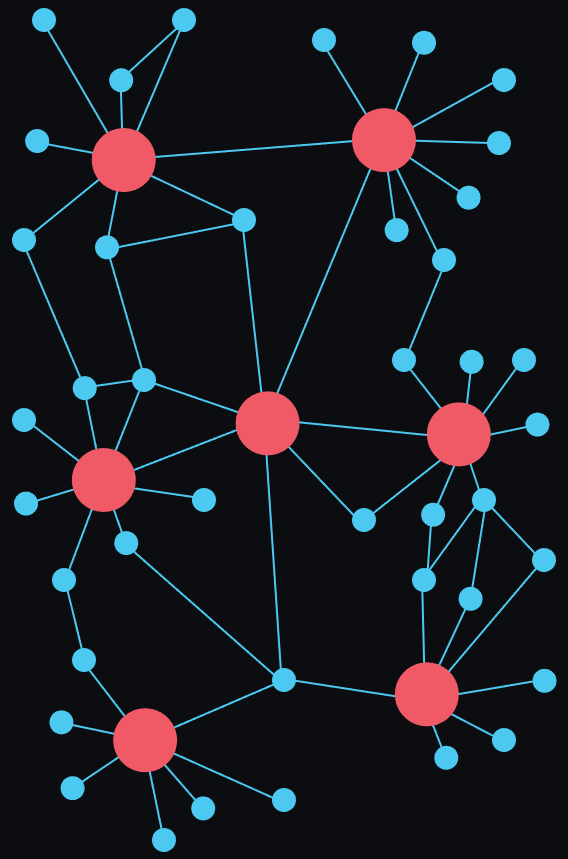
\includegraphics[width=0.19\textwidth]{slide4b.png}}
\hspace{1.2cm}
\subfloat[Decentralizovan]{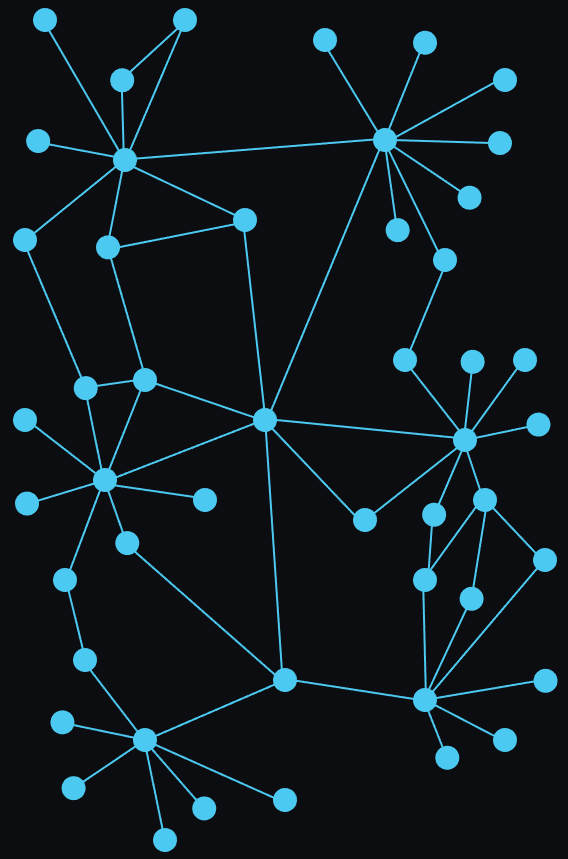
\includegraphics[width=0.19\textwidth]{slide4c.png}}

\caption{Arhitektonski modeli organizacije i upravljanja informacionim sistemima.}
\end{figure}

\end{frame}

% =========================================================
% SLIDE 5
% =========================================================

\begin{frame}{Savremeni informacioni sistemi}

Savremeni informacioni sistemi visokog kapaciteta proširuju kapacitet dodavanjem instanci i raspodelom opterećenja.

Iako je infrastrukturno distribuiran, sistem zadržava centralizovan model upravljanja kroz \redColor{klijent-server komunikaciju} zasnovanu na \redColor{lokacijskom adresiranju}.

Zato je potrebno uvesti model komunikacije zasnovan na \blueColor{mreži ravnopravnih čvorova} (\emph{peer-to-peer}), koji sistem čini otvorenim za učešće.

Koordinacija se ostvaruje algoritmima konsenzusa, među kojima su i deterministički BFT algoritmi zasnovani na razmeni poruka i glasanju između čvorova.

\metodologijaProblem{} Performanse opadaju sa porastom broja čvorova usled povećanja komunikacionog opterećenja.

\end{frame}

\end{document}